\documentclass[11pt]{article}

\usepackage{listings}
\usepackage{xargs}
\PassOptionsToPackage{hyphens}{url}\usepackage{hyperref}
\usepackage{multirow}
\usepackage{tabularx}
\usepackage{subfig}
\usepackage{times}
\usepackage{graphicx}
\usepackage{makecell}
\usepackage{arydshln}
\usepackage{xspace}
\usepackage{deauthor}

\newcommand{\Hypercallback}{Hyperupcall\xspace{}}
\newcommand{\hypercallback}{hyperupcall\xspace{}}
\newcommand{\hide}[1]{}

\begin{document}

\title{Leveraging Hyperupcalls To Bridge The Semantic Gap: An Application Perspective}

\date{}

\author{
{\rm Michael Wei}\\
VMware Research
\and
{\rm Nadav Amit}\\
VMware Research
} 

\maketitle

\begin{abstract}

Hyperupcalls are a mechanism which we recently proposed
to bridge the semantic gap between a hypervisor
and its guest virtual machines (VMs) by allowing the guest VM
to provide the hypervisor safe, verifiable code to transfer information.
With a hyperupcall, a hypervisor can safely read and update data
structures inside the guest, such as page tables. A hypervisor could
use such a hyperupcall, for example, to determine which pages are
free and can be reclaimed in the VM without invoking it.

In this paper, we describe hyperupcalls and how they have been used
to improve and gain additional insight on virtualized workloads. We
also observe that complex applications such as databases hold a
wealth of semantic information which the systems they run on top of
are unaware of. For example, a database may store records, but the
operating system can only observe bytes written into a file, and the
hypervisor beneath it blocks written to a disk, limiting the optimizations the
system may make: for instance, if the operating system understood the database
wished to fetch a database record, it could prefetch related records.
We explore how mechanisms like hyperupcalls could be used from
the perspective of an application, and demonstrate two use cases from an application
perspective: one to trace events in both the guest and hypervisor simultaneously and 
another simple use case 
where a database installs a hyperupcall so the hypervisor can prioritize
certain traffic and improve response latency.

\end{abstract}

\section{Introduction}
\label{sec:introduction}

Previously, we have described Hyperupcalls~\cite{amit2018design}, a tool used to bridge the \emph{semantic gap} in virtualization,
where one side of an abstraction (virtual machines) must be oblivious to the other (hypervisors). The abstraction of a virtual machine (VM), enables
hosts known as \emph{hypervisors} to run multiple operating systems (OSs) known as \emph{guests} simultaneously, 
each under the illusion that they are running in their own physical machine. This is achieved
by exposing a hardware interface which mimics that of true, physical hardware. 
The introduction of this simple abstraction has led to the rise of the modern data center and the cloud as we know it today. Unfortunately,
virtualization is not without drawbacks. Although the goal of virtualization is for VMs and hypervisors to be oblivious from each other, this separation renders both sides unable to understand
decisions made on the other side, a problem known as the semantic gap. 

The semantic gap is not limited to virtualization - it exists whenever an abstraction is used, since the purpose of
the abstraction is to hide implementation details. For example, in databases, a SQL query has limited insight into how
the query planner may execute it, and the query planner has limited insight into the application that sent the SQL
query. Insight into the application may help the database execute the query optimally. If the database 
could see that an application was overloaded, it might be able to delay execution of the query and use the resources
for other applications. Likewise, if the application could see that a column was being reindexed, it may perform
the query on another column, or defer that query for later. 

In virtualization, addressing the semantic gap is critical for performance. Without information about  
decisions made in guests, hypervisors may suboptimally allocate resources. For example,
the hypervisor cannot know what memory is free in guests without understanding their
internal OS state, breaking the VM abstraction. As a result, in virtualized environments, many
mechanisms have been developed to bridge the semantic gap.
State-of-the-art hypervisors today typically bridge the semantic gap
with \emph{paravirtualization}~\cite{barham03,russell08virtio}, 
which makes the guest aware of the hypervisor. Several paravirtual mechanisms exist 
and are summarized in Table~\ref{table:comm}. Another mechanism hypervisors may
leverage is \emph{introspection}, which enables the hypervisor to observe the behavior of
virtual machines without prior coordination. 

% Paravirtualization alleviates the guest from the limitations of the physical hardware interface 
% and allows direct information exchange with the hypervisor, improving overall performance by 
% enabling the hypervisor to make better resource allocation decisions. Paravirtualization, however, involves the execution of code both in the context of the 
% hypervisor and the guest. \emph{Hypercalls} require that the guest make a request to
% be executed in the hypervisor, much like a system call, and \emph{upcalls} require
% that the hypervisor make a request to be executed in the guest. This design introduces
% a number of drawbacks. First, paravirtual mechanisms introduce context switches between
% hypervisors and guests,  which may be substantial if frequent interactions between  
% guests and the hypervisor are needed~\cite{babu2014system}. Second, the requestor of a 
% paravirtual mechanism must wait for it to be serviced in another context which may be
% busy, or waking the guest if it is idle. Finally, paravirtual mechanisms
% couple the design of the hypervisor and guest: paravirtual mechanisms need to be
% implemented for each guest and hypervisor, increasing complexity~\cite{specifications17microsoft} 
% and hampering maintainability~\cite{wuelfing09kroah}. Adding paravirtual features 
% requires updating both the guest and hypervisor with a new interface~\cite{open-vm-tools}
% and has the potential to introduce bugs and the attack surface~\cite{milenkoski2014experience,wojtczuk16windows}.
% A different class of techniques, VM introspection (VMI)~\cite{garfinkel2003virtual} and the reverse, 
% hypervisor introspection (HVI)~\cite{wang2015hypervisor} aim to address some of the
% shortcomings of paravirtualization by \emph{introspecting} the other context, 
% enabling communication transfer without context switching or prior coordination.
% These techniques however, are fragile: small changes in data structures, behavior
% or even security hardening~\cite{hussein17randomization} can break introspective 
% mechanisms, or worse, introduce security vulnerabilities.   
% As a result, introspection is usually relegated to the area of
% intrusion detection systems (IDSs) which detect malware or misbehaving applications.

Each one of these mechanisms used in virtualization may be used elsewhere where the semantic gap exists. For example,
a paravirtual mechanism such as a hypercall might be similar to an application informing a database using an RPC call, whereas an upcall may involve
a database informing an application about it's internal state. While introspection would be more complicated to implement
in the context of applications such as databases, one can imagine a database attempting to infer the workload of
an application by measuring its query rate, or an application trying to determine if a database is overloaded by
measuring response latency.

In this paper, we describe the design and implementation of \hypercallback{}s
\footnote{\Hypercallback{s} were previously published as
	``hypercallbacks''~\cite{amit2017hypercallbacks}.}, 
a technique which enables a hypervisor to communicate with a guest, like an upcall,
but without a context switch, like VMI. This is achieved through the use of verified
code, which enables a guest to communicate to the hypervisor in a flexible manner
while ensuring that the guest cannot provide misbehaving or malicious 
code. Once a guest registers a \hypercallback, the hypervisor can execute
it to perform actions such as locating free guest pages or running guest interrupt handlers
without switching into the guest. We believe that hyperupcalls are useful from the perspective
of an application - both as a tool for an application such as a database to gain insight about 
its clients, and for applications to use in a virtualized environment, breaking the semantic gap
between the application, guest operating system and hypervisor. 

\Hypercallback{}s are easy to build: they are written in a high level language such as C,
and we provide a 
framework which allows \hypercallback{}s to share the same codebase and 
build system as the Linux kernel that may be generalized to other operating systems. 
When the kernel is compiled, a toolchain translates the \hypercallback~into 
verifiable bytecode. This enables \hypercallback{}s to be easily maintained. 
Upon boot, the guest registers the \hypercallback{}s with the hypervisor, 
which verifies the bytecode and compiles it back into native 
code for performance. Once recompiled, the hypervisor may invoke the \hypercallback{} at any time.

We have previously shown that hyperupcalls enable a hypervisor to be proactive about resource
allocation when memory is overcommitted, enhance performance when interprocessor interrupts (IPIs)
are used, and enhance the security and debuggability of systems in virtual environments~\cite{amit2018design}.
In this paper, we show an application use case: we design a hyperupcall which is installed by
memcached to prioritize the handling and reduce the latency of certain requests. 

% This paper makes the following contributions:

% \begin{itemize}

% \item We build a taxonomy of mechanisms for bridging the semantic gap between hypervisor and guests and place \hypercallback{}s within that taxonomy (\S\ref{sec:background}).

% \item We describe and implement \hypercallback{}s (\S\ref{sec:architecture}) with:

% \begin{itemize}
% 	\item An environment for writing \hypercallback{}s and a framework for using guest code (\S\ref{sec:building})
	
% 	\item A compiler (\S\ref{sec:compilation}) and verifier (\S\ref{sec:verification}) for \hypercallback{}s which addresses the complexities and limitations of verified code.
	
% 	\item Registration (\S\ref{sec:registration}) and execution (\S\ref{sec:execution}) mechanisms for \hypercallback{}s.
% \end{itemize}

% \item We prototype and evaluate \hypercallback{}s and show a new application-oriented use case which allows the hypervisor to safely interpret application traffic and re-prioritize the virtual machine, improving latency for high-priority requests.

% \end{itemize}


\section{Communication Mechanisms}
\label{sec:background}

It is now widely accepted that in order to extract the most 
performance and utility from virtualization, hypervisors 
and their guests need to be aware of one another.
To that end, a number of mechanisms exist to facilitate 
communication between hypervisors and guests. Table~\ref{table:comm} 
summarizes these mechanisms, which can be broadly characterized by
the requestor, the executor, 
and whether the mechanism requires that the hypervisor
and the guest coordinate ahead of time. We note that many of these
mechanisms have analogs in other places where the semantic gap may exist.
For example, a hypercall might be similar to a query notification in a database, and
an upcall might resemble an out-of-band request to a service. 

In the next section, we discuss these mechanisms 
and describe how \hypercallback{}s fulfill a need for a 
communication mechanism where the hypervisor makes and 
executes its own requests without context switching. 
We begin by introducing state-of-the-art paravirtual
mechanisms in use today. 


\begin{table}[t]
 \centering
  \small
  \hspace*{-0.4cm}
   \begin{tabular}{clrr|r}
  % & \multicolumn{1}{c}{} &  \multicolumn{3}{c}{\textbf{Coordination \& Execution}}\\
    \parbox[t]{-2mm}{\multirow{4}{*}{\rotatebox[origin=c]{90}{\textbf{Requestor}}}} & \multicolumn{1}{c|}{}& \multicolumn{2}{c}{\textbf{Paravirtual, Executed by}:} & \multicolumn{1}{|c}{\textbf{Uncoordinated}}\\
    & \multicolumn{1}{c|}{}& \multicolumn{1}{c|}{Hypervisor} & \multicolumn{1}{c}{Guest} & \multicolumn{1}{|c}{Introspection}\\
    \cline{2-5}
   & \multicolumn{1}{c|}{Guest} & \multicolumn{1}{c|}{\emph{Hypercalls}} & \multicolumn{1}{c}{Pre-Virt~\cite{levasseur2005pre}} & \multicolumn{1}{|c}{HVI~\cite{wang2015hypervisor}}\\
     \cline{2-5}
   & \multicolumn{1}{c|}{HV} & \multicolumn{1}{c|}{\textbf{\Hypercallback{}s}} & \multicolumn{1}{c}{\emph{Upcalls}} & \multicolumn{1}{|c}{VMI~\cite{garfinkel2003virtual}}\\
   \end{tabular}
   \caption{\emph{Hypervisor-Guest Communication Mechanisms.} Hypervisors (HV) and guests may communicate through a variety of mechanisms, which are characterized by who initiates the communication, who executes and whether the channel for communication is coordinated (paravirtual).
    \emph{Italicized} cells represent channels which require context switches. }
  \label{table:comm}
   \end{table}
  
\subsection{Paravirtualization}

\paragraph{Hypercalls and upcalls.} Most hypervisors today leverage paravirtualization to communicate across 
the semantic gap. Two mechanisms in widespread use today are \emph{hypercalls},
which allow guests to invoke services provided by the hypervisor, and 
\emph{upcalls}, which enable the hypervisor to make requests to guests.
Paravirtualization means that the interface for these mechanisms are coordinated ahead of time between
hypervisor and guest~\cite{barham03}.

One of the main drawbacks of upcalls and hypercalls is that they
require a context switch as both mechanisms are executed on the opposite
side of the request. As a result, these
mechanisms must be invoked with care. Invoking a hypercall or upcall
too frequently can result in high latencies and computing resource 
waste~\cite{amit11}. 

Another drawback of upcalls in particular that the requests are
handled by the guest, which could be busy handling other tasks. If the
guest is busy or if a guest is idle, upcalls incur
the additional penalty of waiting for the guest to be free or
for the guest or woken up. This can take an unbounded amount of time,
and hypervisors may have to rely on a penalty system to ensure guests
respond in a reasonable amount of time.

Finally, by increasing the coupling between the hypervisor and its guests,
paravirtual mechanisms can be difficult to maintain over time. Each hypervisor
have their own paravirtual interfaces, and each guest must implement the interface
of each hypervisor. The paravirtual interface is not thin: Microsoft's paravirtual interface specification
 is almost 300 pages long~\cite{specifications17microsoft}. Linux provides a variety of paravirtual hooks, 
 which hypervisors can use to communicate with the VM~\cite{xenparavirtops}. 
 Despite the effort to standardize the paravirtualization interfaces they are incompatible with each other, and
 evolve over time, adding features or even removing some (e.g., Microsoft hypervisor event tracing). As a result, most hypervisors do not
 fully support efforts to standardize interfaces and specialized OSs look for alternative solutions~\cite{madhavapeddy2013unikernels,porter11rethinking}.

 \paragraph{Pre-virtualization.} Pre-Virtualization~\cite{levasseur2005pre} is another mechanism 
 in which the guest requests services from the hypervisor, but the requests are served in the 
 context of the guest itself. This is achieved by code injection: the guest leaves stubs, which the 
 hypervisor fills with hypervisor code. Pre-virtualization offers an improvement over hypercalls, 
 as they provide more flexible interface between the guest and the hypervisor. Arguably, pre-virtualization suffers
 from a fundamental limitation: code that runs in the guest is deprivileged and cannot perform
 sensitive operations, for example, accessing shared I/O devices. As a result, in pre-virtualization, 
 the hypervisor code that runs in the guest still needs to communicate with
 the privileged hypervisor code using hypercalls.

\subsection{Introspection}
Introspection occurs when a hypervisor or guest attempts to infer information from
the other context without directly communicating with it. With introspection, no
interface or coordination is required. For instance, a hypervisor may attempt to
infer the state of completely unknown guests simply by their memory access patterns.
Another difference between introspection and paravirtualization is that no context
switch occurs: all the code to perform introspection is executed in the requestor.

\paragraph{Virtual machine introspection (VMI).} When a hypervisor introspects a guest, it is known as VMI~\cite{garfinkel2003virtual}. 
VMI was first introduced to enhance VM security by 
providing intrusion detection (IDS) and kernel integrity checks from a privileged 
host~\cite{baliga2011detecting, fu2012space, garfinkel2003virtual}. 
VMI has also been applied to checkpointing and deduplicating VM state~\cite{aderholdt2014efficient}, 
as well as monitoring and enforcing hypervisor policies~\cite{ranadive2009ibmon}. 
These mechanisms range from simply observing a VM's memory and I/O access patterns~\cite{jones2006antfarm} 
to accessing VM OS data structures~\cite{case2010dynamic}, and at the extreme end they may modify VM state and 
even directly inject processes into it~\cite{gu2011process, chiueh2012surreptitious}. The primary benefits of 
VMI are that the hypervisor can directly invoke VMI without a context switch, 
and the guest does not need to be ``aware'' that it is inspected for VMI to function. 
However, VMI is fragile: an innocuous change in the VM OS, such as a hotfix which adds an additional
field to a data structure could render VMI non-functional~\cite{bahram2010dksm}.
As a result, VMI tends to be a ``best effort'' mechanism.

\paragraph{HVI.} Used to a lesser extent, a guest may introspect the hypervisor it is running on, 
known as hypervisor introspection (HVI)~\cite{wang2015hypervisor, shi2016hardware}. HVI is
 typically employed either to secure a VM from untrusted hypervisors~\cite{shih2016s} or by
  malware to circumvent hypervisor security~\cite{rutkowska08,mishra2017intrusion}.
  %it could also be used by an altruistic VM to release resources when a hypervisor is under pressure, or to optimize I/O access patterns.
%In the hypervisor, this is known as virtual machine introspection (VMI)~\cite{garfinkel2003virtual}. VMI was first introduced to enhance VM security by providing intrusion detection (IDS) and kernel integrity checks from a privileged host-mode~\cite{baliga2011detecting, fu2012space, garfinkel2003virtual, hofmann2011ensuring, ibrahim2011cloudsec, jiang2007stealthy, payne2008lares}. VMI has also been applied to checkpointing and deduplicating VM state~\cite{aderholdt2014efficient, chiang2013introspection, wood2007black}, as well as monitoring and enforcing hypervisor policies~\cite{baig2014cloudflow, hizver2014real, ranadive2009ibmon, suneja2014non}. These mechanisms range from simply observing a VM's memory and I/O access patterns~\cite{jones2006antfarm, chen2001virtual} to accessing VM OS data structures~\cite{case2010dynamic}, and at the extreme end, they may modify VM state and even directly inject processes into it~\cite{gu2011process, chiueh2012surreptitious}. The primary benefits of VMI are that the hypervisor can directly invoke VMI in order to respond to an event without running the VM, and the VM does not need to be ``aware'' that is inspected for VMI to function. However, VMI is fragile: an innocuous change in the VM OS, such as a hotfix which adds an additional field to a data structure could render VMI non-functional, or worse, a malicious VM OS could craft state to mislead or potentially crash the hypervisor~\cite{bahram2010dksm}. As a result, VMI tends to be a ``best effort'' mechanism.

\hide{
Introspection is also used, to a lesser extent, from the VM OS to learn about the hypervisor it is running on, known as hypervisor introspection (HVI)~\cite{wang2015hypervisor, shi2016hardware}. While HVI is typically employed either to secure a VM from an untrusted hypervisor~\cite{shih2016s} or by malware to circumvent hypervisor security mechanisms~\cite{rutkowska08,mishra2017intrusion}, it could also be used by an altruistic VM to release resources when a hypervisor is under pressure, or to optimize I/O access patterns.
}


\subsection{Extensible OSes}
While hypervisors provide a fixed interface, OS research suggested along the years
that flexible OS interfaces can improve performance without sacrificing security. The Exokernel
provided low level primitives, and allowed applications to implement high-level abstractions,
for example for memory management~\cite{engler1995exokernel}. SPIN allowed to extend kernel
functionality to provide application-specific services, such as specialized interprocess
communication~\cite{bershad1995extensibility}. The key feature that enables these extensions
to perform well without compromising security, is the use of a simple byte-code to express
application needs, and running this code at the same protection ring as the kernel.
Our work is inspired by these studies, and we aim to design a flexible interface between the hypervisor
and guests to bridge the semantic gap.

\subsection{\Hypercallback{}s}

This paper introduces \hypercallback{}s, which fulfill a need for a mechanism
for the hypervisor to communicate to the guest which is coordinated (unlike VMI),
executed by the hypervisor itself (unlike upcalls) and does not require context switches (unlike hypercalls).
With \hypercallback{}s, the VM coordinates with the hypervisor by registering verifiable code. 
This code is then executed by the hypervisor in response to events (such as memory pressure, or VM entry/exit). In
a way, \hypercallback{}s can be thought of as upcalls executed by the hypervisor.

\begin{figure}[t!]
	\centering
	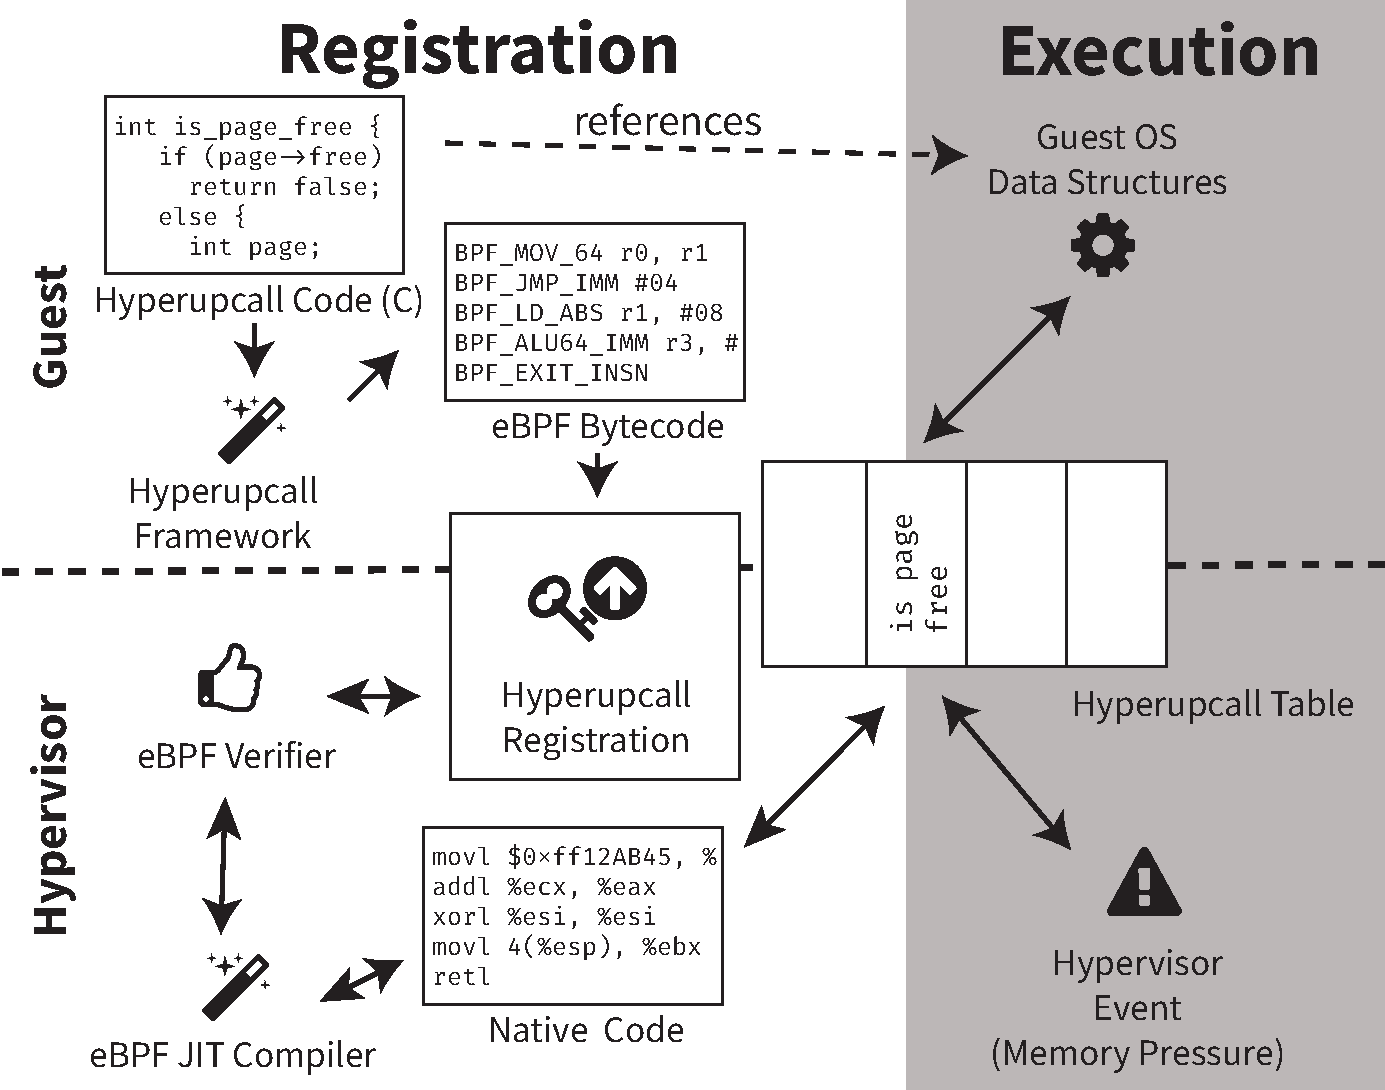
\includegraphics[width=\columnwidth]{figs/architecture.pdf}
	\caption{\emph{System Architecture.} \Hypercallback{} registration (left) consists of 
	compiling C code, which may reference guest data structures, into verifiable bytecode. 
	The guest registers the generated bytecode with the hypervisor, which verifies its safety, 
	compiles it into native code and sets it in the VM \hypercallback~table. When the 
	hypervisor encounters an event (right), such as a memory pressure, it executes the respective 
	\hypercallback, which can access and update data structures of the guest.}
	\label{fig:system_overview}
    \end{figure}
    
In contrast to VMI, the code to access VM state is provided by the guest 
so the \hypercallback{}s are fully aware of guest internal data structures---
in fact, \hypercallback{}s are built with the guest OS codebase and share the same code, 
thereby simplifying maintenance while providing the OS with an expressive mechanism to 
describe its state to underlying hypervisors. 

Compared to upcalls, where the hypervisor makes asynchronous requests to the guest, 
the hypervisor can execute a \hypercallback{} at any time, even when the guest is not running. 
With an upcall, the hypervisor is at the mercy of the guest, which may delay the upcall~\cite{arya2014tesseract}. 
Furthermore, because upcalls operate like remote requests, upcalls may be forced to implement OS functionality in 
a different manner. For example, when flushing remote pages in memory ballooning~\cite{waldspurger2002memory}, 
the canonical technique for identifying free guest memory,
the guest increases memory pressure using a dummy process to free pages. With a \hypercallback, 
the hypervisor can act as if it were a guest kernel thread and scan the guest for free pages directly.

\Hypercallback{}s resemble pre-virtualization, in that code is transferred across the semantic gap. Transferring code not only allows for more expressive communication, but it also moves the execution of the request to the other side of the gap, enhancing performance and functionality. Unlike pre-virtualization, the hypervisor cannot trust the code being provided by the virtual machine, and the hypervisor must ensure that execution environment for the \hypercallback~is consistent across invocations.

In some ways, hyperupcalls may resemble SQL stored procedures: they are a block of code installed across
the semantic gap, and code is more expressive than a simple request. One important distinction between
hyperupcalls and stored procedures is that hyperupcalls have access to the guest state and data structures,
whereas stored procedures do not. This allows hyperupcalls to be much more expressive and dynamic compared
to simple code transfer mechanisms.

    
\section{Architecture}
\label{sec:architecture}


%Hyperupcalls consist of writing, registration, and execution.
%let's detail these in order.


% What are hyperupcalls?
\Hypercallback{}s are short verifiable programs provided by
guests to the hypervisor to improve performance 
or provide additional functionality. Guests provide \hypercallback{s}
to the hypervisor through a \emph{registration} process at boot, allowing
the hypervisor to access the guest OS state and provide services by \emph{executing} them
after verification. The hypervisor runs \hypercallback{}s 
in response to events or when it needs to
query guest state. The architecture
of \hypercallback{}s and the system we have built for utilizing them is depicted in Figure~\ref{fig:system_overview}.

We aim to make \hypercallback{}s as simple as possible to build. To that end, 
we provide a complete \emph{framework} which allows a programmer to write
\hypercallback{}s using the guest OS codebase. This greatly simplifies the development and maintenance of 
\hypercallback{}s. The framework compiles this code into verifiable code which the
guest registers with the hypervisor. In the next section, we describe how an OS
developer writes a \hypercallback~using our framework. Some of the implementation details, especially in regards
to how we verify that the code is safe and execute the hyperupcall, are out of the scope of this paper. For more details, see~\cite{amit2018design}.

%. The programs, however, needs to be self-contained
%and cannot call any external code of the VM. The high-level
%language is compiled into simple byte-code, whose safety
%can be relatively easily determined.

%The VM OS registers
%the hyperupcalls after boot, and defines which of the
%predefined hypervisor events triggers each program.

% memory+close cooperation
%Although hyperupcalls run in the hypervisor world, they appear to 
%run in the VM kernel address-space and can be written to access 
%VM data using pointers in the guest virtual address (GVA) space.
%As a result, and since they are written in a high-level language,
%they can share code with the VM OS. These characteristics allow
%them to closely cooperate with other mechanisms of the VM OS.
%Compiler enhancements and the VM OS framework make the development
%of hyperupcalls simple.

% Limitations premier
%%While hyperupcalls resemble any OS code, they do have certain
%limitations, as they need to be verifiable.
%Moreover, they can only access
%a subset of the VM virtual address space, which is guaranteed
%not to be constant.

\subsection{Building \Hypercallback{}s}
\label{sec:building}
% Overview

Guest OS developers write \hypercallback{}s for each hypervisor event
they wish to handle. Hypervisors and guests agree on these events, for example  
VM entry/exit, page mapping or virtual CPU (VCPU) preemption.
Each \hypercallback{} is identified by a predefined identifier, much
like the UNIX system call interface~\cite{ritchie1978unix}. 

\subsubsection{Providing Safe Code}

One of the key properties of \hypercallback{}s is that the code
must be guaranteed to not compromise the hypervisor. In order
for a \hypercallback{} to be safe, it must only be able to access a
restricted memory region dictated by the hypervisor, 
run for a limited period of time without blocking,
sleeping or taking locks, and only use hypervisor services that
are explicitly permitted.

Since the guest is untrusted, hypervisors must rely on
a security mechanism which guarantees these safety properties. There are many
solutions that we could have chosen: software fault isolation (SFI)~\cite{wahbe1994efficient},
proof-carrying code~\cite{necula1997proof} or safe languages such as Rust. 
To implement \hypercallback{s}, we chose the enhanced Berkeley Packet Filter (eBPF) VM.

We chose eBPF for several reasons. First, eBPF is relatively mature: 
BPF was introduced over 20 years ago and is used extensively 
throughout the Linux kernel, originally for packet filtering but
extended to support additional use cases such as 
sandboxing system calls (\texttt{seccomp}) and tracing of kernel 
events~\cite{bcc}. eBPF enjoys wide adoption and is supported by various 
runtimes~\cite{bigswitch15ubpf,monnet17rbpf}.
Second, eBPF can be provably verified to have the safety properties we
require, and Linux ships with a verifier and JIT which verifies 
 and efficiently executes eBPF code~\cite{wang2014jitk}.
Finally, eBPF has a LLVM compiler backend, which enables eBPF bytecode 
to be generated from a high level language using a compiler frontend
(Clang). Since OSes are typically written in C, the eBPF LLVM backend 
provides us with a straightforward mechanism to convert unsafe guest OS source 
code into verifiably safe eBPF bytecode. 

\subsubsection{From C to eBPF --- the \emph{Framework}}

Unfortunately, writing a \hypercallback{} is not as simple recompiling
OS code into eBPF bytecode. However, our 
framework aims to make the process of writing a \hypercallback{s} simple and 
maintainable as possible. The framework provides three key features that simplify 
the writing of \hypercallback{s}. First, the framework takes care of dealing with 
guest address translation issues so guest OS symbols are available to the 
\hypercallback. Second, the framework addresses limitations of eBPF, 
which places significant constraints on C code. Finally, the framework 
defines a simple interface which provides the \hypercallback{} with data so 
it can execute efficiently and safely.

\paragraph{Guest OS symbols and memory.} Even though \hypercallback{}s have access 
to the entire physical memory of the guest, accessing guest OS data structures
 requires knowing where they reside.
OSes commonly use kernel address space layout randomization (KASLR) to randomize
the virtual offsets for OS symbols, 
rendering them unknown during compilation time. Our framework enables OS symbol 
offsets to be resolved at runtime by associating pointers %with different sections 
using address space attributes and injecting code to adjust the pointers.
When a \hypercallback~is registered, the guest provides the actual symbol 
offsets enabling a \hypercallback~developer to reference OS symbols 
(variables and data structures) in C code as if they were accessed by a kernel thread.
% Since global \hypercallback{s}
%must complete their execution in a timely manner, we ensure that for these
% callbacks the guest OS pages requested are pinned during the \hypercallback, 
% and restrict the memory that can be accessed to 2\% of the guest's total 
% physical memory (this setting may be configured).
% TODO: THIS IS NOT REQUIRED FOR LOCAL

\paragraph{Global / Local \Hypercallback{s}.} Not all \hypercallback{s} need 
to be executed in a timely manner. For example, notifications informing the 
guest of hypervisor events such as a VM-entry/exit or interrupt injection 
only affect the guest and not the hypervisor. We refer to  \hypercallback{s} 
that only affect the guest that registered it as local, and \hypercallback{s} 
that affect the hypervisor as a whole as global. If a \hypercallback{} is 
registered as local, we relax the timing requirement and allow the 
\hypercallback{} to block and sleep. Local \hypercallback{s} are accounted 
in the vCPU time of the guest similar to a trap, so a misbehaving \hypercallback{} 
penalizes itself. 

Global \hypercallback{s}, however, must complete their execution in a timely manner. 
We ensure that for the guest OS pages requested by global \hypercallback{}s are 
pinned during the \hypercallback, and restrict the memory that can be accessed 
to 2\%  (configurable) of the guest's total physical memory.
Since local \hypercallback{s} may block, the memory
 they use does not need to be pinned, allowing local \hypercallback{s}
  to address all of guest memory.


\paragraph{Addressing eBPF limitations.} While eBPF is 
expressive, the safety guarantees of eBPF bytecode mean that it is not
 Turing-complete and limited, so only a subset of C 
 code can be compiled into eBPF. The major limitations of eBPF are 
 that it does not support loops, the ISA does not contain atomics,
  cannot use self-modifying code, function pointers, static variables, 
  native assembly code, and cannot be too long and complex to be verified.

One of the consequences of these limitations is that \hypercallback{} 
developers must be aware of the code complexity of the \hypercallback, 
as complex code will fail the verifier. While this may appear to be an 
unintuitive restriction, other Linux developers using BPF face the same 
restriction, and we provide a helper functions in our framework 
to reduce complexity, such as \texttt{memset} and \texttt{memcpy}, as well as
functions that perform native atomic operations such as \texttt{cmpxchg}. 
A selection of these helper functions is shown in Table~\ref{table:helpers}.
In addition, our framework masks memory accesses~(\S\ref{sec:verification}), 
which greatly reduces the complexity of verification. In practice, as
long as we were careful to unroll loops, we did not encounter verifier 
issues while developing the use cases in~(\S\ref{sec:evaluation}) using 
a setting of 4096 instructions and a stack depth of 1024.

%\paragraph{eBPF security.} The safety of eBPF is cornerstone to the design of the \hypercallback. While helper functions increase the potential attack surface into the
%hypervisor, they tend to be small ($<$ 10 SLOC), and are a part of the eBPF specification and used throughout Linux in perf, pcap and iptables. The inputs to the helper functions are verified before they are used. In addition, the Linux eBPF JIT engine was exploited (and patched) as a result of the Spectre vulnerability~\ref{spectre}. \Hypercallback{s} 

\paragraph{\Hypercallback{} interface.} When a hypervisor invokes a \hypercallback,
it populates a context data structure, shown in Table~\ref{table:context}. The
\hypercallback{} receives an \texttt{event} data structure which indicates the reason
the callback was called, and a pointer to the guest (in the address space of the hypervisor,
which is executing the \hypercallback). When the \hypercallback{} completes, it may return a
value, which can be used by the hypervisor.

\paragraph{Writing the \hypercallback.} With our framework, OS developers write C code 
which can access OS variables and data structures, assisted by the helper functions of
the framework. A typical \hypercallback{} will read the \texttt{event} field, read or update
OS data structures and potentially return data to the hypervisor. Since the 
\hypercallback{} is part of the OS, the developers can reference the same data
structures used by the OS itself---for example, through header files. This greatly 
increases the maintainability of \hypercallback{s}, since data layout changes 
are synchronized between the OS source and the \hypercallback{} source. 

It is important to note that a \hypercallback{} cannot invoke guest OS functions 
directly, since that code has not been secured by the framework. However, 
OS functions can be compiled into \hypercallback{}s and be integrated in 
the verified code.


%First,  \hypercallback{}s have access to the full virtual address space
%of the VM OS, known as the \emph{guest virtual address} (GVA),
%OS security mechanisms
%such as kernel address space layout randomization (KASLR)
%may render symbol addresses unknown at compilation time, as
%\hypercallback{}s are not linked to the kernel. Allowing \hypercallback{}s
%to access these symbols easily is critical for
%simplifying \hypercallback~development, allowing developers to access 
%VM OS data structures as if the \hypercallback~were running on a VM OS 
%kernel thread.  To support this, our framework 
%extracts the symbol addresses before KASLR and creates a
%header file with preprocessor macros to provide
%the symbol addresses. These macros set an address-space attribute
%for symbols from different sections, and the eBPF compiler uses
%these attributes to inject code that performs the required address translations.

%In addition, eBPF places
%significant limitations on C, and common features of VM OS
%code, such as native assembly instructions, loops, or 
%static variables are prohibited. To overcome these limitations, 
%\hypercallback~developers can use
%our framework, which provides verifiable implementations of
%common OS functions. For example, in Linux, the function that
%sets a bit non-atomically on the x86 architecture uses the 
%\texttt{bts} assembly instruction, and is replaced by simple 
%C code in our framework. In other cases, however, the 
%verifiable bytecode cannot provide equivalent
%functionality, and our framework invokes
%hypervisor helper functions to provide the
%same functionality. Some examples for helper functions are given in
%Table~\ref{table:helpers}. The verifier can check that the inputs
%to the helper function are valid, but it is up to the 
%helper function to make sure that it is safe (for example, sanitizing
%inputs and performing bound checks). Typically, helper functions
%are short and call pre-existing functions in the hypervisor.

\begin{table}[t!]
 \centering
 \small
 \begin{tabular}{c|l}
 \textbf{Helper Name} & \textbf{Function} \\
 \hline
 \texttt{send\_vcpu\_ipi} & Send an interrupt to VCPU \\
 \texttt{get\_vcpu\_register} & Read a VCPU register\\
 \texttt{set\_vcpu\_register} & Read a VCPU register\\
 \texttt{memcpy} & \texttt{memcpy} helper function \\
 \texttt{memset} & \texttt{memset} helper function \\
 \texttt{cmpxchg} & compare-and-swap \\
 \texttt{flush\_tlb\_vcpu} & Flush VCPU's TLB \\
 \texttt{get\_exit\_info} &  Get info on an \texttt{VM\_EXIT} event
 \end{tabular}
 \caption{\emph{Selected \hypercallback~helper functions.} The \hypercallback{} may call these functions implemented in the hypervisor, as they cannot be verified using eBPF.}
\label{table:helpers}
 \end{table}

\begin{table}[t!]
 \centering
 \small
 \begin{tabularx}{\columnwidth}{c|X}
 \textbf{Input field} & \textbf{Function} \\
 \hline
 \texttt{event} & Event specific data including event ID. \\
 \texttt{hva} & Host virtual address (HVA) in which the guest memory is mapped. \\
 \texttt{guest\_mask} & Guest address mask to mask bits which are higher than
	the guest memory address-width. Used for verification (\S\ref{sec:verification}).\\
 \texttt{vcpus} & Pointers to the hypervisor VCPU data structure, if
	the event is associated with a certain VCPU, or a pointer
	to the guest OS data structure. Inaccessible to the
	hyperupcall, but used by helper functions.\\
 \texttt{vcpu\_reg} & Frequently accessed VCPU registers: instruction pointer and VCPU ID. \\
 \texttt{env} & Environment variables, provided by the guest
	during \hypercallback registration. Used to set address randomization offsets. \\
 \end{tabularx}
 \caption{\emph{\Hypercallback~context data}. These fields are populated by the hypervisor when a \hypercallback~is called.}
\label{table:context}
 \end{table}
 
\hide{
\begin{figure}[!t]
\begin{lstlisting}[basicstyle=\scriptsize\ttfamily,language=C,                keywordstyle=\color{blue}\ttfamily,
                stringstyle=\color{red}\ttfamily,
                commentstyle= \color{ForestGreen}\ttfamily]
int is_page_free(struct hcb_page __host *hp)
{
     unsigned long gfn = hdp->gpa >> PAGE_SHIFT;
     struct page *page = pfn_to_page(gfn);
     unsigned int order;
 
#pragma unroll
     for (order = 0; order < MAX_ORDER; order++) {
          struct page *page_head = 
             page - (pfn & ((1 << order) - 1));
 
          if (PageBuddy(page_head) 
          	 && page_order(page_head) >= order)
                  break;
     }
     return order < MAX_ORDER;
}
\end{lstlisting}
  \caption{\emph{Page free \hypercallback.} This Linux \hypercallback~checks if a VM OS page is free.
  All functions used, such as \texttt{pfn\_to\_page} and \texttt{PageBuddy} are Linux kernel functions.}
\label{fig:bpf_example}
\end{figure}
}

%Overall, our framework makes it easy to build \hypercallback{}s.
%%For example, in Linux the code to detect whether a page is free is identical
%to the the function \texttt{is\_free\_buddy\_page}, excluding the loop unrolling directive, which
%is necessary to make the code verifiable.
\hide{
Next, we discuss to inputs and outputs of a \hypercallback,
as well as a \hypercallback's limitations.
}


\hide{
Hyperupcalls are short VM programs, which run as 
callbacks in the host context when certain hypervisor events 
are triggered. Hyperupcalls are 
provided with an input argument that is called ``context'', which
describes the event that triggered the callback. The hyperupcall
can then perform computations, read and write VM memory, and
invoke certain hypervisor helper functions. Finally, program
that are registered on ``query'' events return to the hypervisor
answers for the queries.

% high-level language
Hyperupcalls can be written in high-level language, such as C,
which allows the callback to share the same code-base with the
VM OS. This can simplify the development and maintenance of 
hyperupcalls. The programs, however, needs to be self-contained
and cannot call any external code of the VM. The high-level
language is compiled into simple byte-code, whose safety
can be relatively easily determined.
}



%\paragraph{Hyperupcall inputs.}
%Before the hypervisor invokes a hyperupcall, it provides 
%the hyperupcall a ``context'' data structure, which describes the
%occurring event, as well as environment variables, which were
%defined by the VM during registration.
%This data structure holds event-specific data, but shares
%a mutual base structure, which includes the following
%components:

%\paragraph{Helper Functions.}
%% problem
%The simplicity of eBPF comes with a cost: eBPF cannot be used for
%common operations. The limited instruction-set does not support
%atomic operations, for instance compare-and-swap, or memory
%barriers. To simplify verification, the eBPF verifier does not
%allow the use of loops, which complicates the implementation
%of common functions, for example \texttt{memcpy}.
%Moreover, hyperupcalls often need to perform additional tasks
%which are unique to hyperupcalls, and unsupported by eBPF.
%For example, hyperupcalls need to read or write VCPU registers,
%or inject an interrupt into a VCPU.
%
%% helper functions
%To overcome these limitations, eBPF allows the privileged 
%entity---the hypervisor in our case---to define external
%``helper functions'', which the eBPF program is allowed
%to call. The hypervisor defines an API of helper functions
%that can be used by hyperupcalls.
%
%\paragraph{Framework.}
%% Extending per type
%We develop a small framework for incorporating
%existing OS (Linux) code in hyperupcalls, which
%provides alternative implementations of common OS functions that cannot
%be verified, since the implementation uses native assembly instructions,
%loops, or static variables.
%The framework provides verifiable, although potentially less
%efficient implementation. For example, the Linux function that
%sets a bit non-atomically on the x86 architecture uses the \texttt{bts}
%assembly instruction, and is replaced by simple C code in our framework. In
%other cases, however, the verifiable byte-code cannot provide an equivalent
%functionality, and our framework invokes
%host helper functions to provide the
%same functionality.
%
%In addition, our framework solves the use of OS symbols by
%hyperupcalls, as hyperupcalls are not linked and the symbol addresses
%are unknown during compilation if the OS uses kernel address space
%layout randomization (KASLR). The framework extracts the symbol addresses
%before KASLR and creates a header file with preprocessor macros to provide
%the symbol addresses. These macros set an address-space attribute
%for symbols from different sections. As we present in \cref{sec:compilation},
%the compiler uses these attributes to generate code that performs the necessary
%address translations.
%
%\paragraph{Return value.}
%The hyperupcalls API defines which of the events are notifications,
%whose return value is ignored, and which are queries, and how the
%hypervisor regards the return value. For example, a hyperupcall that is
%registered on an ``exit'' event, which is triggered after the 
%hypervisor traps a VM event, returns whether the trapped event
%was handled by the hyperupcall. If it was handled, the hypervisor
%resumes the VCPU without running its standard exit-handlers. In 
%Figure~\ref{fig:bpf_example}, the \hypercallback indicates
%whether the page can be discarded and returns 1 if it
%is unused by the VM OS.

%\paragraph{Hyperupcall limitations and events.}
%Running native OS code in hyperupcalls requires several adaptations
%to make the code verifiable. The code needs to be self-contained
%for the verifier to ensure its safety.
%Consequently, building hyperupcall requires the refactoring of the OS
%code to extract functionality which is used both by the VM OS and
%hyperupcall into separate source files.
%In addition, for the code to be compiled and verified successfully,
%it cannot use self-modifying code, function pointers, static variables,
%native assembly code, and cannot be too long and complex to be verified.
%
%% Loop unroll
%One of the notable limitation is the restriction on using loops
%as they cannot be verified. There are several ways to address this
%limitation. Our framework overrides common functions
%that use loops, such as \texttt{memcpy} and \texttt{memset}
%with calls to helper functions that provide the same functionality.
%Yet, in other cases, the OS code needs to be adapted to avoid loops in
%hyperupcall. If loops are used for small number of iterations,
%a compiler directive can be used to unroll it.  
%Some loops can be safely removed when the
%code runs in hyperupcall, as they are intended with events 
%that cannot happen while the hyperupcall runs, for instance VM 
%interrupts.
%Otherwise, the code needs to be adapted to fail gracefully if loop
%is needed.
%
%Another important limitation is that hyperupcalls can only access
%memory whose mappings, from GVA to guest physical address (GPA),
%do not change. This limitation is due to the complexity and overheads
%of synchronizing the VM and the hypervisor
%memory mappings. If the VM needs to access data using a memory
%mapping which is not fixed, it needs to run code that 
%performs a page-walk and converts the address, if possible, into
%an address with fixed mappings.


%\paragraph{Event Types.}
%The hypervisor defines events in which the hyperupcalls of the VM
%are be called. Each event is categorized as either local or global
%event.
%
%Some extra limitations apply for certain events the hypervisor
%uses to make global policy decisions, since they must be executed
%in a timely manner. Table~\ref{table:events} distinguishes these global
%events from local events and summarizes the limitations, which we detail
%by event type:
%
%\emph{Local Events.}
%The vast majority of \hypercallback~events are local. These events
%are VM-specific events that do not affect other VMs.
%Local events are only triggered when a VCPU of
%the VM is running and the callbacks are executed in the context of the hypervisor
%thread that runs a VCPU. Their execution time is accounted as part of the VM
%runtime, just as the time that the hypervisor spends handling VM
%traps is accounted.
%
%% Notifications limitation
%Since poor performance of local event \hypercallback{}s only affects the VM that 
%registered it, the hypervisor does not need to
%set strict limitations.
%The runtime of these \hypercallback{}s does not
%need to be tightly bounded, as the hypervisor can preempt them and schedule a
%different VCPU of another VM. As a result, the hypervisor
%allows these \hypercallback{}s to block due to paging, and does not pin the callback
%memory. In addition, the hypervisor allows the VM to chain events by
%registering multiple callbacks on each event.
%
%% Notification virtual memory limits
%Running the \hypercallback~in the context of the VCPU allows us to map the \hypercallback~
%memory in the address space of the hypervisor userspace process that handles the
%VM. In addition, the registered memory does not need to be pinned, as
%page faults the occur during the \hypercallback~can be treated as other page faults
%that occur when the hypervisor accesses the VM memory.
%As a result, the size of the memory the \hypercallback~can use 
%does not need to be strictly limited.
%Since mapping the memory still consumes hypervisor resources, especially
%the page tables that map the callback memory, the hypervisor may
%still limit the memory that is accessible for these callbacks. For
%example, the limit may be set to the VM physical memory.
%
%\emph{Global Events.}
%In contrast to local events, global events can be triggered when a VCPU
%is suspended or about to be preempted. Global events are triggered
%when global resource allocation operations occur such as memory
%reclamation or VCPU preemption, and provide information to the hypervisor
%that assist resource allocation decisions. Since these decisions 
%must be made in a timely manner, \hypercallback{}s that are registered on
%global events must complete and provide an answer within a short 
%bounded time.
%
%% What we need 
%The hypervisor places stricter limits on \hypercallback{}s which register on 
%global events. First, the \hypercallback~memory cannot be paged out since this 
%may cause unbounded delay. Second, the memory must be 
%constantly mapped in the hypervisor kernel page-tables to avoid the overhead of
%page-faults and switching address spaces before running the callback.
%The hypervisor fulfills these two requirements by ensuring the memory
%that the VM uses for the hyperupcall is relatively small. 
%Finally, helper functions
%whose execution time may be long cannot be invoked on global events.
%The hypervisor ensures this property is fulfilled during the program
%verification.
%
%\hide{
%% packed + inline
%Finally, the eBPF compiler imposes some requirements.
%eBPF requires all the code to be inlined, which requires
%all functions to use the \texttt{always\_inline} attribute.
%Packed structure in LLVM prevent the compiler from ensuring the alignment
%of memory accesses~\cite{song17packed}, which results in complex and inefficient
%code. The adaptation of the code is eased by using preprocessor macros.
%}

\hide{vmalloc, memory hot-add}

\subsection{Compilation}
\label{sec:compilation}

Once the \hypercallback{} has been written, it needs to be compiled into
eBPF bytecode before the guest can register it with the hypervisor. Our
framework generates this bytecode as part of the guest OS build process by
running the \hypercallback~C code through Clang and the eBPF LLVM backend,
with some modifications to assist with address translation and verification:



%The hyperupcall source code is compiled into a verifiable byte-code.
%In our implementation we use the LLVM compiler with its eBPF backend
%for this matter. To allow hyperupcalls to reuse existing OS code
%and seamlessly
%run in the hypervisor, we extend the compiler to perform the required
%transformation to the generated byte-code.

\paragraph{Guest memory access.}

To access guest memory, we use eBPF's direct packet 
access (DPA) feature, which was designed to allow programs to access network
packets safely and efficiently without the use of helper functions.
Instead of passing network packets, we utilize this feature by treating the 
 guest as a ``packet''. Using DPA in this manner required a bug 
 fix~\cite{amit17llvm} to the eBPF LLVM backend, as it was written with
 the assumption that packet sizes are $\leq$64KB.


\paragraph{Address translations.}
% in our design?

\Hypercallback{}s allow the hypervisor to seamlessly use guest virtual
addresses (GVAs), which makes it
appear as if the \hypercallback{} was running in the guest. However, the code is actually executed by the
hypervisor, where host virtual address (HVAs) are used, rendering guest pointers invalid.
To allow the use of guest pointers transparently in the host context, these pointers therefore
need to be translated from GVAs into HVAs. We use the compiler to make these translations.

To make this translation simple, the hypervisor maps the GVA range contiguously
in the HVA space, so address translations can easily be done by adjusting the base address.
As the guest might need the \hypercallback{} to access multiple contiguous GVA 
ranges---for example, one for the guest 1:1 direct mapping and of the OS text section~\cite{kleen04map}---our framework
annotates each pointer with its respective ``address space'' attribute. We extend the LLVM compiler
to use this information to inject eBPF code that converts each of the pointer from
GVA to HVA by a simple subtraction operation. It should be noted that the generated code safety
is not assumed by the hypervisor and is verified when the \hypercallback{} 
is registered.

\hide{
, which is provided in the \texttt{hdp}
parameter shown in Figure~\ref{fig:bpf_example}. 
}

%One of the main features of hyperupcalls is the ability to seamlessly 
%use GVAs, as if the code runs in the VM. However,
%as we show next~(\ref{sec:registration}),
%the host maps the hyperupcall memory contiguously, but
%in a different virtual
%address range. This limitation is inherent, as different VMs
%might, and are even likely, to use overlapping GVA ranges
%for their hyperupcalls.

%% translation during compilation
%We therefore enhance the LLVM compiler to generate eBPF code
%that performs  required translations during compilation of
%hyperupcalls. The compiler inserts instructions 
%to add an offset to the GVAs, which is given in the hyperupcall
%input. This offset is actually given by the VM when the hyperupcall
%is registered, and the hypervisor forwards it to the hyperupcall,
%when it is invoked.
%Since the hyperupcall may also use HVAs, specifically for
%accessing the ``context'' input, we use the compiler's address-space 
%attributes to distinguish between GVA pointers and HVA ones.
%The compiler is set to generate code to translate GVAs
%and leave HVAs intact. We set the GVA space as zero,
%which is the default one, to allow to incorporate 
%unmodified OS code in hyperupcalls.

%Actually, the hyperupcall
%code can access GVAs in different contiguous ranges. For example,
%in the Linux hyperupcalls that we created, most pointers are
%in Linux's direct mappings address range, while the variables
%are in the text section (which alias part of the direct
%mappings address range)~\cite{kleen04map}. As we mentioned
%before, the framework marks the variable with a different
%address-space attribute, which allows the compiler to set
%the correct offset for addresses in the different sections.

\paragraph{Bound Checks.}
The verifier rejects code with direct memory accesses unless it can ensure
the memory accesses are within the ``packet'' (in our case, guest memory) bounds.
We cannot expect the \hypercallback{} programmer to perform the required checks, 
as the burden of adding them is substantial. We therefore enhance the compiler 
to automatically add code that performs bound checks prior to each memory access,
allowing verification to pass. As we note in Section~\ref{sec:verification}, 
the bounds checking is done using masking and not branches to ease verification.

%As we present in \cref{sec:verification}, instead of adding checks
%that the accesses are valid and branching accordingly, 
%we set the compiler to mask the offset in the registered memory.

\paragraph{Context caching.}
Our compiler extension introduces 
intrinsics to get a pointer to the context or to read its data. The context
is frequently needed along the callback for calling helper functions
and for translating GVAs. Delivering the context
as a function parameter requires intrusive 
changes and can prevent sharing code between the guest and its \hypercallback.
Instead, we use the compiler to cache the context pointer in one of the registers
and retrieve it when needed.


\subsection{Registration}
\label{sec:registration}

After a \hypercallback{} is compiled into eBPF bytecode, it is ready to
be registered. Guests can register \hypercallback{}s at any time, but
most \hypercallback{}s are registered when the guest boots. The guest
provides the \hypercallback{} event ID, \hypercallback~bytecode and 
the virtual memory the \hypercallback~will use. 

\subsection{Verification}
\label{sec:verification}

The hypervisor verifies that each \hypercallback{} is safe to
execute at registration time. Our verifier is based on the Linux 
eBPF verifier and checks three properties of the \hypercallback: 
memory accesses, number of runtime instructions, and helper functions
used. 


\subsection{Execution}
\label{sec:execution}

Once the hyperupcall is compiled, registered and verified, it may be executed by the hypervisor in response to an event.
There are some complexities to executing hyperupcalls, for accessing remote CPU states and dealing with locks. In general, the hypervisor can run the hyperupcall to obtain information about
the guest without waiting on a response from the guest.

%!TEX root = paper.tex

\section{Use Cases and Evaluation}
\label{sec:evaluation}
Previously, we presented several use cases for hyperupcalls which primarily involved the guest operating system: enabling a hypervisor to be proactive about resource
allocation when memory is overcommitted, enhancing performance when interprocessor interrupts (IPIs)
are used, and increasing the security and debuggability of systems in virtual environments~\cite{amit2018design}. From the 
application perspective, we also provided a modified version of the \texttt{ftrace} utility to help application developers
see both hypervisor and guest events in a unified view. In this section, we focus on the application use cases
of hyperupcalls: first we present both the frace utility previously presented and a new use case where
we enable memcached to install a hyperupcall to prioritize certain traffic. This enables the hypervisor
to safely understand application traffic and perform actions based on application state without coupling
the hypervisor with application code.

\subsection{Unified Event Tracing}
% Why it is important
Event tracing is an important tool for debugging correctness
and performance issues. However, collecting traces for virtualized workloads 
is somewhat limited. Traces collected
inside a guest do not show hypervisor events, such as when a VM-exit is forced,
 which can have significant
effect on performance. For traces that are collected in the hypervisor
to be informative, they require knowledge about guest OS symbols~\cite{carbone14vprobes}. 
Such traces cannot be collected in cloud environments. In addition,
each trace collects only part of the events and does
not show how guest and hypervisor events interleave.

% Our solution
To address this issue, we run the Linux kernel tracing tool, \texttt{ftrace}~\cite{ftrace},
inside a \hypercallback. \texttt{Ftrace} is well suited to run in a \hypercallback. 
It is simple, lockless,
and built to enable concurrent tracing in multiple contexts: non-maskable
interrupt (NMI), hard and soft interrupt handlers and user processes.
As a result, it was easily be adapted to trace hypervisor events
 concurrently with guest events.
Using the \texttt{ftrace} \hypercallback, the guest can trace both hypervisor
and guest events in one unified log, easing debugging. Since tracing
all events use only guest logic, new OS versions can change the tracing logic, without requiring
hypervisor changes. 

Tracing is efficient, despite the \hypercallback
complexity (3308 eBPF instructions), as most of the code deals
with infrequent events that handles situations in which trace
pages fill up. Tracing using  \hypercallback{}s is slower than using
native code by 232 cycles, which
is still considerably shorter time than the time a context switch between the
hypervisor and the guest takes.

Tracing is a useful tool for performance debugging, which can
expose various overheads~\cite{zheng2009warp}. For example, 
by registering the \texttt{ftrace} on the VM-exit event, we see
that many processes, including short-lived ones, trigger multiple
VM exits due to the execution of the \texttt{CPUID} instruction, 
which enumerates the CPU
features and must be emulated by the hypervisor. We found
that the GNU C Library, which is
used by most Linux applications, uses \texttt{CPUID} 
to determine the supported CPU features. This overhead 
could be prevented by extending Linux virtual dynamic shared 
object (vDSO) for applications to query the supported CPU features
without triggering an exit.

\subsection{Scheduler Activation}
Our scheduler activation hyperupcall prototype performs scheduler activation by increasing the virtual
machine priority for a short time when a packet which matches a condition arrives
to the guest. memcached registers a hyperupcall with the guest, which in turn registers a
hyperupcall with the hypervisor on a guest packet receiving event. In our prototype implemetation, 
this hyperupcall simply boosts the VM priority using a helper function, but we could have
also performed other actions such as inspect the packet contents or access guest data structures.
We increase the VM priority (\texttt{cpu.weight}) from a default value of 10 to 100 for 100ms.


\begin{figure*}
	\includegraphics[width=\textwidth]{figs/memcached_sched-eps-converted-to.pdf}
	\caption{The runtime of 100 memcached requests with varying
	level of CPU overcommitment, with and without scheduler activation
	hyperupcalls. The slowdown ratio is presented above the lines.}
	\label{fig:sched}
\end{figure*}

Figure~\ref{fig:sched} shows the results. We used a memcached server in a guest with a single VCPU
and increased the level of overcommittment of the physical CPU the machine was running on.
The guest and multiple background tasks (iperf)
were executed in different \texttt{cgroups} with equal priority. We assume
in our experiment that the same user owns all the different guests. A workload generator (memcslap) was dispatched every second to issue 100 requests to the VM.
Each experiment as conducted 50 times and the average execution time and standard deviation are shown.

Overall, this use case demonstrates that an application can use hyperupcalls to prioritize requests to the
guest in an application-specific manner, greatly reducing latency and variability. We believe that we have
only scratched the surface, and there are many other use cases of hyperupcalls which can be used to enhance
applications. Since hyperupcalls can seamlessly integrate into the codebase of the application and are able to
access guest state, developing new use cases is greatly simplified. We are currently working on making
it easier for the hyperupcall to access application state, as well as methods for the guest OS to safely
register multiple hyperupcalls on the same event.

\section{Availability}
\label{sec:availability}

We are in the process of open sourcing the hyperupcalls infrastructure and intend to make it available to the public soon. 
In the meantime, interested parties may contact the authors to obtain a pre-release version. Currently, the hyperupcalls
infrastructure we intend to release is built for Linux virtual machines, and is integrated into the source code of the
Linux kernel. Additional work is necessary to fully expose this interface to other applications.

There are several contexts which the hyperupcalls infrastructure could be used in other applications. An application wishing
to install its own hyperupcalls, as in the example use cases we developed, could do so using an interface provided 
by the operating system. However, the operating system would need to have a mechanism for multiplexing hyperupcalls
registered to the same event, or not support multiplexing at all. Another context that hyperupcalls could be used
by applications is for applications to use the hyperupcalls concept of running verified trusted code. Our infrastructure
does not yet support this, but could serve as an example system for leveraging eBPF in applications to run code to 
bridge the semantic gap.

\section{Conclusion}
\label{sec:conclusion}

Bridging the semantic gap is critical for performance and for the hypervisor to
provide advanced services to guests. Hypercalls and upcalls are currently used to
bridge the gap, but they have several drawbacks: hypercalls cannot be initiated 
by the hypervisor, upcalls do not have a bounded runtime, and both incur the
penalty of context switches. Introspection,
an alternative which avoids context switches can be unreliable as it relies on
observations instead of an explicit interface. \Hypercallback{}s overcome 
these limitations by allowing the guest to expose its \emph{logic} to the hypervisor,
avoiding a context switch by enabling the \hypercallback{} to safely execute guest
logic directly.


We have built a complete infrastructure for developing \hypercallback{}s which
allow developers to easily add new paravirtual features using the codebase of the OS. This
infrastructure could easily be extended to be used by applications as well, enabling
applications to provide the hypervisor insight into their internal state. They can also be 
used to bridge the semantic gap outside of virtualization, for example, for services such
as databases to gain more insight about the applications which use them.

\begin{thebibliography}{10} 
  \itemsep=1pt 
  \begin{small}

  \bibitem{aderholdt2014efficient}
  Ferrol Aderholdt, Fang Han, Stephen~L Scott, and Thomas Naughton.
  \newblock Efficient checkpointing of virtual machines using virtual machine
    introspection.
  \newblock In {\em IEEE/ACM International Symposium on Cluster, Cloud and Grid
    Computing (CCGrid)}, pages 414--423, 2014.
  
  \bibitem{amit17llvm}
  Nadav Amit.
  \newblock Patch: Wrong size-extension check in {BPFDAGToDAGISel::SelectAddr}.
  \newblock
    \url{https://lists.iovisor.org/pipermail/iovisor-dev/2017-April/000723.html},
    2017.
  
  \bibitem{amit11}
  Nadav Amit, Muli Ben-Yehuda, Dan Tsafrir, and Assaf Schuster.
  \newblock {vIOMMU}: efficient {IOMMU} emulation.
  \newblock In {\em USENIX Annual Technical Conference (ATC)}, 2011.
  
  \bibitem{amit2018design}
  Nadav Amit and Michael Wei.
  \newblock The design and implementation of hyperupcalls.
  \newblock In {\em 2018 USENIX Annual Technical Conference (ATC)}, pages
    97--112, 2018.
  
  \bibitem{amit2017hypercallbacks}
  Nadav Amit, Michael Wei, and Cheng-Chun Tu.
  \newblock Hypercallbacks: Decoupling policy decisions and execution.
  \newblock In {\em ACM Workshop on Hot Topics in Operating Systems (HOTOS)},
    pages 37--41, 2017.
  
  \bibitem{arya2014tesseract}
  Kapil Arya, Yury Baskakov, and Alex Garthwaite.
  \newblock Tesseract: reconciling guest {I/O} and hypervisor swapping in a {VM}.
  \newblock In {\em ACM SIGPLAN Notices}, volume~49, pages 15--28, 2014.
  
  \bibitem{babu2014system}
  Anish Babu, MJ~Hareesh, John~Paul Martin, Sijo Cherian, and Yedhu Sastri.
  \newblock System performance evaluation of para virtualization, container
    virtualization, and full virtualization using {Xen, OpenVX, and Xenserver}.
  \newblock In {\em {IEEE International Conference on Advances in Computing and
    Communications (ICACC)}}, pages 247--250, 2014.
  
  \bibitem{bahram2010dksm}
  Sina Bahram, Xuxian Jiang, Zhi Wang, Mike Grace, Jinku Li, Deepa Srinivasan,
    Junghwan Rhee, and Dongyan Xu.
  \newblock Dksm: Subverting virtual machine introspection for fun and profit.
  \newblock In {\em IEEE Symposium on Reliable Distributed Systems}, pages
    82--91, 2010.
  
  \bibitem{baliga2011detecting}
  Arati Baliga, Vinod Ganapathy, and Liviu Iftode.
  \newblock Detecting kernel-level rootkits using data structure invariants.
  \newblock {\em IEEE Transactions on Dependable and Secure Computing},
    8(5):670--684, 2011.
  
  \bibitem{barham03}
  Paul Barham, Boris Dragovic, Keir Fraser, Steven Hand, Tim Harris, Alex Ho,
    Rolf Neugebauer, Ian Pratt, and Andrew Warfield.
  \newblock Xen and the art of virtualization.
  \newblock In {\em ACM Symposium on Operating Systems Principles (SOSP)}, 2003.
  
  \bibitem{bershad1995extensibility}
  Brian~N Bershad, Stefan Savage, Przemyslaw Pardyak, Emin~G{\"u}n Sirer, Marc~E
    Fiuczynski, David Becker, Craig Chambers, and Susan Eggers.
  \newblock Extensibility safety and performance in the spin operating system.
  \newblock {\em ACM SIGOPS Operating Systems Review (OSR)}, 29(5):267--283,
    1995.
  
  \bibitem{bigswitch15ubpf}
  {Big Switch Networks}.
  \newblock Userspace {eBPF} {VM}.
  \newblock \url{https://github.com/iovisor/ubpf}, 2015.
  
  \bibitem{carbone14vprobes}
  Martim Carbone, Alok Kataria, Radu Rugina, and Vivek Thampi.
  \newblock {VProbes}: Deep observability into the {ESXi} hypervisor.
  \newblock VMware Technical Journal
    \url{https://labs.vmware.com/vmtj/vprobes-deep-observability-into-the-esxi-hypervisor},
    2014.
  
  \bibitem{case2010dynamic}
  Andrew Case, Lodovico Marziale, and Golden~G Richard.
  \newblock Dynamic recreation of kernel data structures for live forensics.
  \newblock {\em Digital Investigation}, 7:S32--S40, 2010.
  
  \bibitem{chiueh2012surreptitious}
  Tzi-cker Chiueh, Matthew Conover, and Bruce Montague.
  \newblock Surreptitious deployment and execution of kernel agents in windows
    guests.
  \newblock In {\em IEEE/ACM International Symposium on Cluster, Cloud and Grid
    Computing (CCGrid)}, pages 507--514, 2012.
  
  \bibitem{engler1995exokernel}
  Dawson~R. Engler, M.~Frans Kaashoek, and James O'Toole~Jr.
  \newblock {\em {Exokernel}: An operating system architecture for
    application-level resource management}, volume~29.
  \newblock 1995.
  
  \bibitem{fu2012space}
  Yangchun Fu and Zhiqiang Lin.
  \newblock Space traveling across vm: Automatically bridging the semantic gap in
    virtual machine introspection via online kernel data redirection.
  \newblock In {\em IEEE Symposium on Security and Privacy (SP)}, pages 586--600,
    2012.
  
  \bibitem{garfinkel2003virtual}
  Tal Garfinkel and Mendel Rosenblum.
  \newblock A virtual machine introspection based architecture for intrusion
    detection.
  \newblock In {\em The Network and Distributed System Security Symposium
    (NDSS)}, volume~3, pages 191--206, 2003.
  
  \bibitem{gu2011process}
  Zhongshu Gu, Zhui Deng, Dongyan Xu, and Xuxian Jiang.
  \newblock Process implanting: A new active introspection framework for
    virtualization.
  \newblock In {\em IEEE Symposium on Reliable Distributed Systems (SRDS)}, pages
    147--156, 2011.
  
  \bibitem{hussein17randomization}
  Nur Hussein.
  \newblock Randomizing structure layout.
  \newblock \url{https://lwn.net/Articles/722293/}, 2017.
  
  \bibitem{bcc}
  {IO Visor Project}.
  \newblock {BCC} - tools for {BPF}-based {Linux} {IO} analysis, networking,
    monitoring, and more.
  \newblock \url{https://github.com/iovisor/bcc}, 2015.
  
  \bibitem{jones2006antfarm}
  Stephen~T Jones, Andrea~C Arpaci-Dusseau, and Remzi~H Arpaci-Dusseau.
  \newblock Antfarm: Tracking processes in a virtual machine environment.
  \newblock In {\em USENIX Annual Technical Conference (ATC)}, pages 1--14, 2006.
  
  \bibitem{kleen04map}
  Andi Kleen.
  \newblock Linux virtual memory map.
  \newblock Linux-4.8:Documentation/x86/x86\_64/mm.txt, 2004.
  
  \bibitem{levasseur2005pre}
  Joshua LeVasseur, Volkmar Uhlig, Matthew Chapman, Peter Chubb, Ben Leslie, and
    Gernot Heiser.
  \newblock {\em Pre-virtualization: Slashing the cost of virtualization}.
  \newblock Universit{\"a}t Karlsruhe, Fakult{\"a}t f{\"u}r Informatik, 2005.
  
  \bibitem{madhavapeddy2013unikernels}
  Anil Madhavapeddy, Richard Mortier, Charalampos Rotsos, David Scott, Balraj
    Singh, Thomas Gazagnaire, Steven Smith, Steven Hand, and Jon Crowcroft.
  \newblock Unikernels: Library operating systems for the cloud.
  \newblock In {\em ACM SIGPLAN Notices}, volume~48, pages 461--472, 2013.
  
  \bibitem{specifications17microsoft}
  Microsoft.
  \newblock Hypervisor top level functional specification v5.0b, 2017.
  
  \bibitem{milenkoski2014experience}
  Aleksandar Milenkoski, Bryan~D Payne, Nuno Antunes, Marco Vieira, and Samuel
    Kounev.
  \newblock Experience report: an analysis of hypercall handler vulnerabilities.
  \newblock In {\em {IEEE International Symposium on Software Reliability
    Engineering (ISSRE)}}, pages 100--111, 2014.
  
  \bibitem{mishra2017intrusion}
  Preeti Mishra, Emmanuel~S Pilli, Vijay Varadharajan, and Udaya Tupakula.
  \newblock Intrusion detection techniques in cloud environment: A survey.
  \newblock {\em Journal of Network and Computer Applications}, 77:18--47, 2017.
  
  \bibitem{monnet17rbpf}
  Quentin Monnet.
  \newblock Rust virtual machine and {JIT} compiler for {eBPF} programs.
  \newblock \url{https://github.com/qmonnet/rbpf}, 2017.
  
  \bibitem{necula1997proof}
  George~C Necula.
  \newblock Proof-carrying code.
  \newblock In {\em ACM SIGPLAN-SIGACT Symposium on Principles Of Programming
    Languages (POPL)}, pages 106--119, 1997.
  
  \bibitem{porter11rethinking}
  Donald~E Porter, Silas Boyd-Wickizer, Jon Howell, Reuben Olinsky, and Galen~C
    Hunt.
  \newblock Rethinking the library {OS} from the top down.
  \newblock In {\em ACM SIGPLAN Notices}, volume~46, pages 291--304, 2011.
  
  \bibitem{ranadive2009ibmon}
  Adit Ranadive, Ada Gavrilovska, and Karsten Schwan.
  \newblock Ibmon: monitoring {VMM}-bypass capable infiniband devices using
    memory introspection.
  \newblock In {\em Workshop on System-level Virtualization for HPC (HPCVirt)},
    pages 25--32, 2009.
  
  \bibitem{ritchie1978unix}
  Dannies~M. Ritchie and Ken Thompson.
  \newblock The {UNIX} time-sharing system.
  \newblock {\em The Bell System Technical Journal}, 57(6):1905--1929, 1978.
  
  \bibitem{ftrace}
  Steven Rostedt.
  \newblock Debugging the kernel using {Ftrace}.
  \newblock LWN.net, \url{http://lwn.net/Articles/365835/}, 2009.
  
  \bibitem{russell08virtio}
  Rusty Russell.
  \newblock virtio: towards a de-facto standard for virtual {I/O} devices.
  \newblock {\em ACM SIGOPS Operating Systems Review (OSR)}, 42(5):95--103, 2008.
  
  \bibitem{rutkowska08}
  Joanna Rutkowska and Alexander Tereshkin.
  \newblock Bluepilling the {X}en hypervisor.
  \newblock {\em BlackHat USA}, 2008.
  
  \bibitem{shi2016hardware}
  Jiangyong Shi, Yuexiang Yang, and Chuan Tang.
  \newblock Hardware assisted hypervisor introspection.
  \newblock {\em SpringerPlus}, 5(1):647, 2016.
  
  \bibitem{shih2016s}
  Ming-Wei Shih, Mohan Kumar, Taesoo Kim, and Ada Gavrilovska.
  \newblock {S-NFV}: Securing {NFV} states by using {SGX}.
  \newblock In {\em ACM International Workshop on Security in Software Defined
    Networks \& Network Function Virtualization (SDN-NFV)}, pages 45--48, 2016.
  
  \bibitem{open-vm-tools}
  VMware.
  \newblock open-vm-tools.
  \newblock \url{https://github.com/vmware/open-vm-tools}, 2017.
  
  \bibitem{wahbe1994efficient}
  Robert Wahbe, Steven Lucco, Thomas~E Anderson, and Susan~L Graham.
  \newblock Efficient software-based fault isolation.
  \newblock In {\em ACM SIGOPS Operating Systems Review (OSR)}, volume~27, pages
    203--216, 1994.
  
  \bibitem{waldspurger2002memory}
  Carl~A Waldspurger.
  \newblock Memory resource management in {VMware ESX} server.
  \newblock {\em ACM SIGOPS Operating Systems Review (OSR)}, 36(SI):181--194,
    2002.
  
  \bibitem{wang2015hypervisor}
  Gary Wang, Zachary~John Estrada, Cuong~Manh Pham, Zbigniew~T Kalbarczyk, and
    Ravishankar~K Iyer.
  \newblock Hypervisor introspection: A technique for evading passive virtual
    machine monitoring.
  \newblock In {\em USENIX Workshop on Offensive Technologies (WOOT)}, 2015.
  
  \bibitem{wang2014jitk}
  Xi~Wang, David Lazar, Nickolai Zeldovich, Adam Chlipala, and Zachary Tatlock.
  \newblock Jitk: A trustworthy in-kernel interpreter infrastructure.
  \newblock In {\em USENIX Symposium on Operating Systems Design \&
    Implementation (OSDI)}, pages 33--47, 2014.
  
  \bibitem{wojtczuk16windows}
  Rafal Wojtczuk.
  \newblock Analysis of the attack surface of {Windows} 10 virtualization-based
    security.
  \newblock BlackHat USA, 2016.
  
  \bibitem{wuelfing09kroah}
  Britta Wuelfing.
  \newblock {Kroah-Hartman}: Remove {Hyper-V} driver from kernel?
  \newblock Linux Magazine
    \url{http://www.linux-magazine.com/Online/News/Kroah-Hartman-Remove-Hyper-V-Driver-from-Kernel},
    2009.
  
  \bibitem{xenparavirtops}
  {Xen Project}.
  \newblock {XenParavirtOps}.
  \newblock \url{https://wiki.xenproject.org/wiki/XenParavirtOps}, 2016.
  
  \bibitem{zheng2009warp}
  Haoqiang Zheng and Jason Nieh.
  \newblock {WARP}: Enabling fast {CPU} scheduler development and evaluation.
  \newblock In {\em IEEE International Symposium On Performance Analysis of
    Systems and Software (ISPASS)}, pages 101--112, 2009.
  \end{small}
  \end{thebibliography}

\end{document}